\section{Условия проведения эксперимента}

	В качестве режущего инструмента принят заостренный дисковый	резец изображенный на рисунке \ref{fig:DRI}.

	% \begin{wrapfigure}{l}{0.5\textwidth}
	%   \vspace{-25pt}
	%   \begin{center}
	%     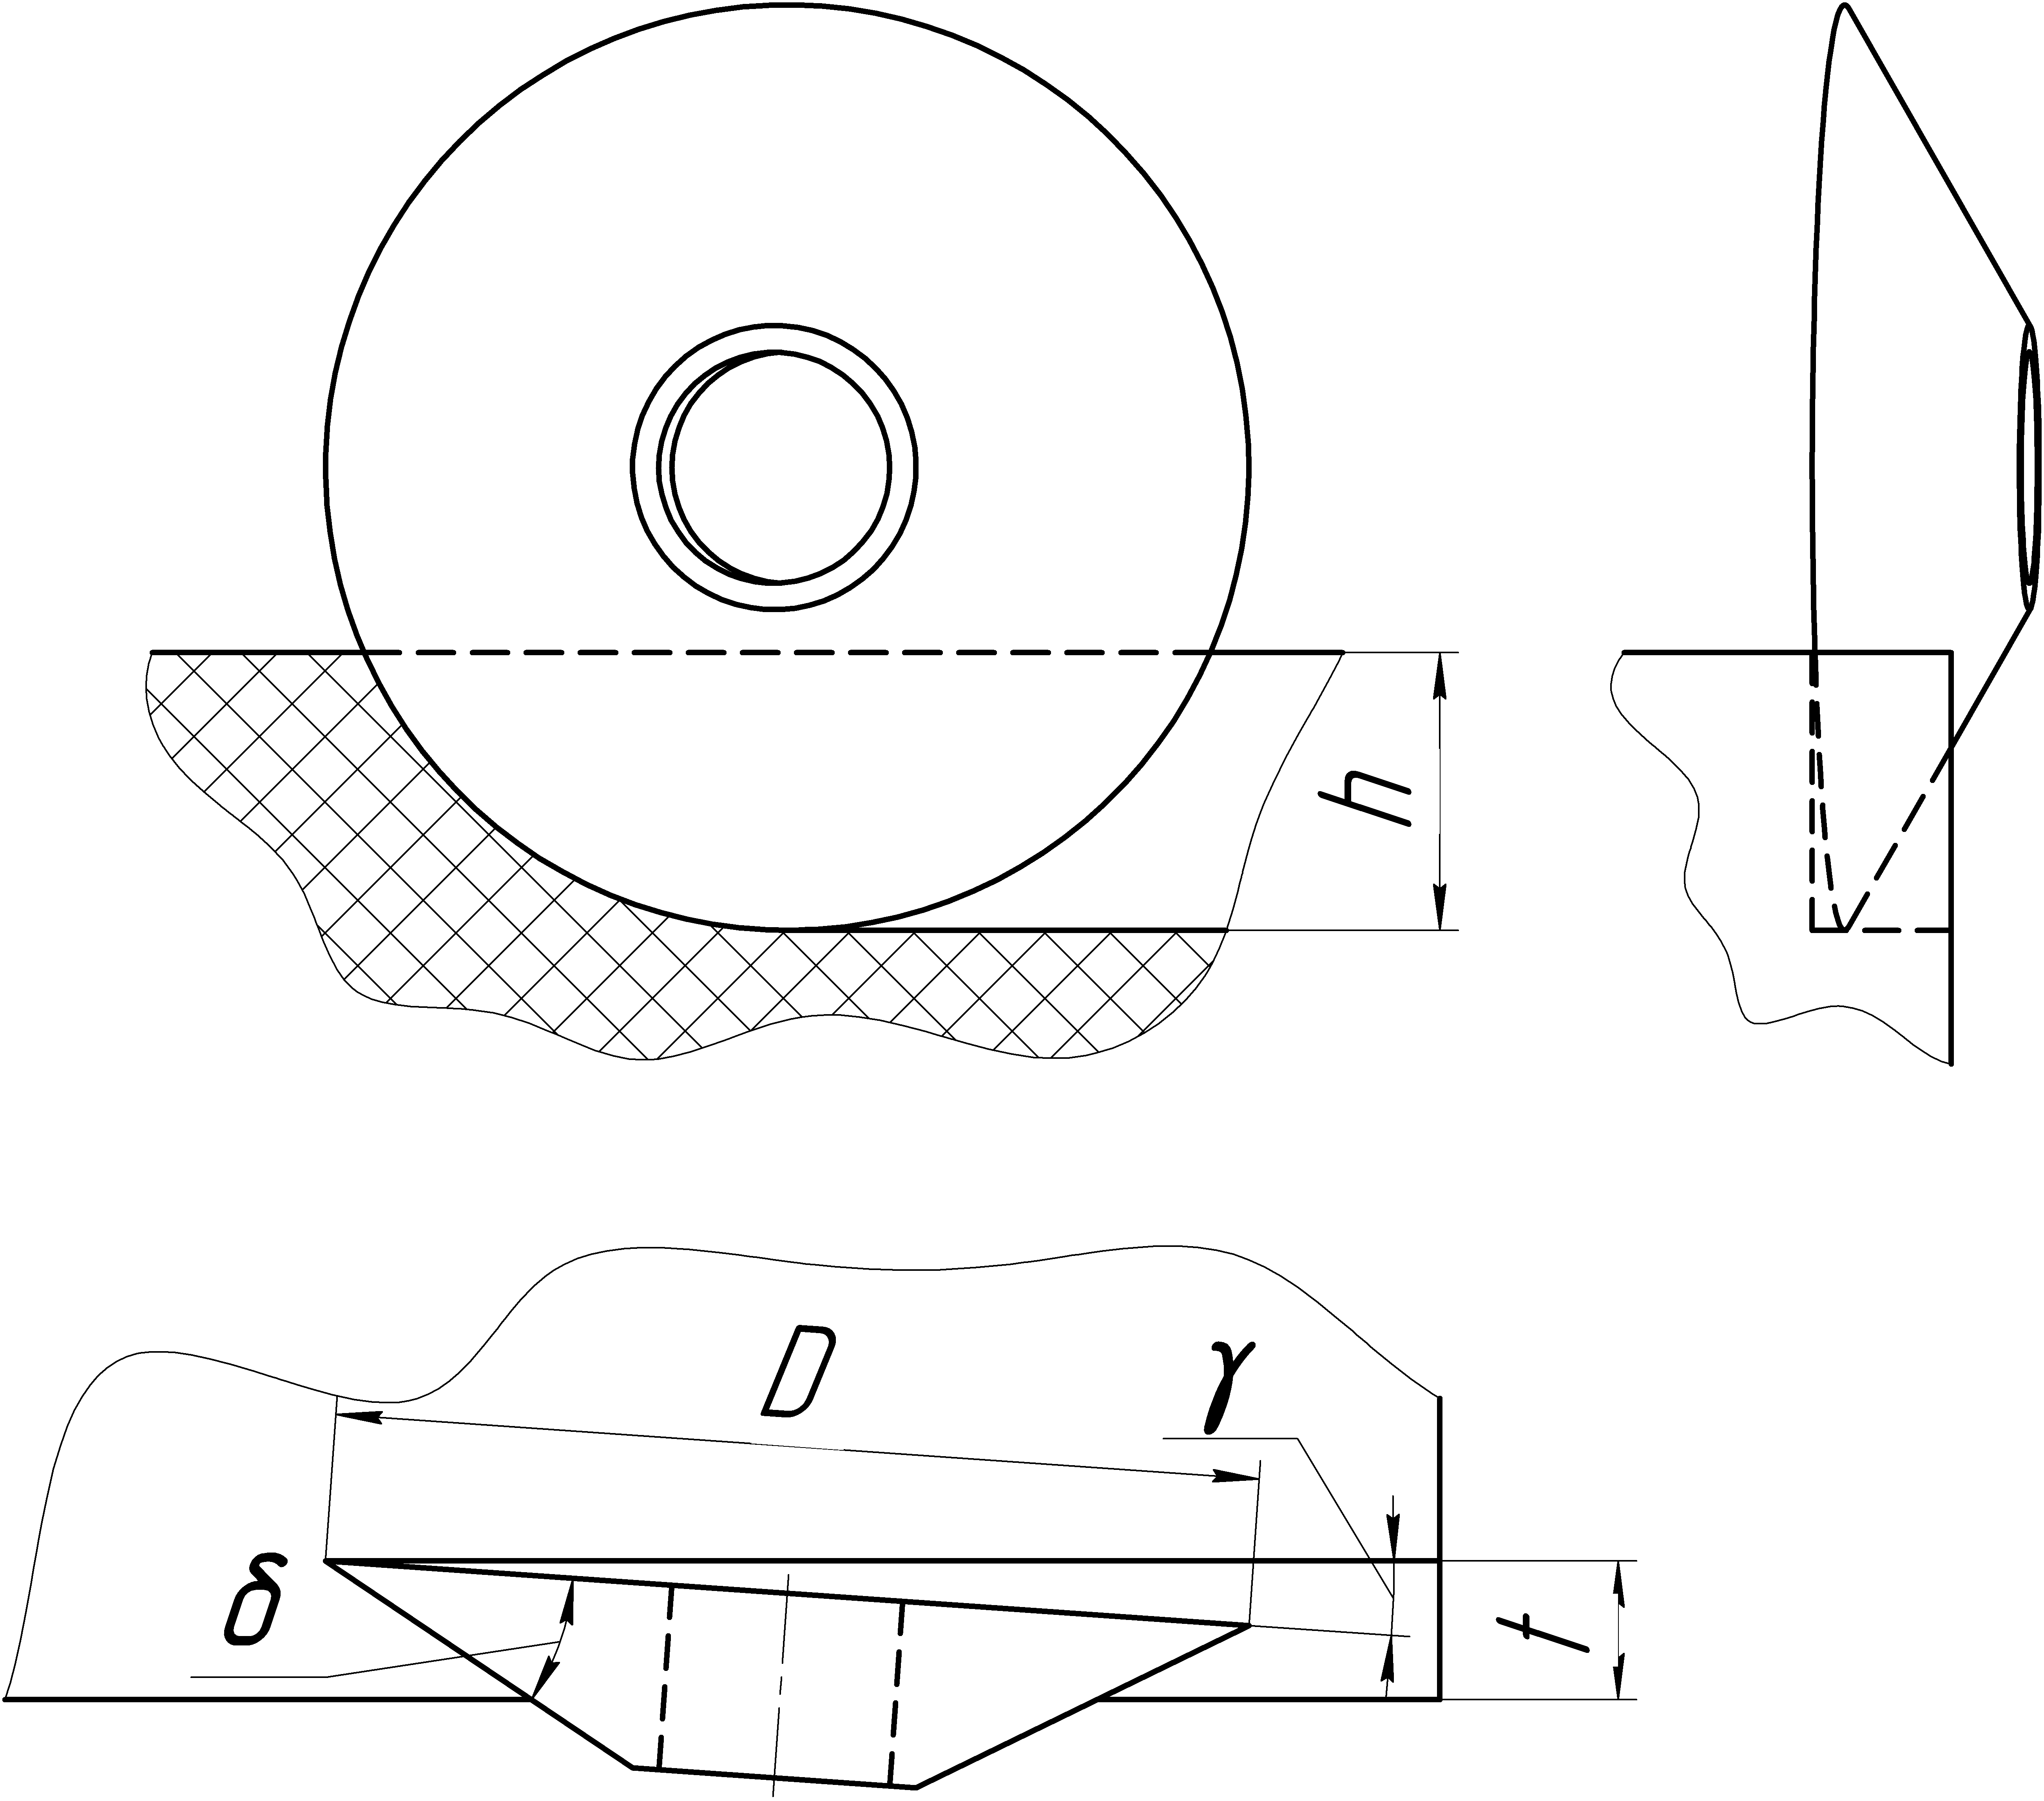
\includegraphics[width=0.5\textwidth]{DRI}
	%   \end{center}
	%   \vspace{-15pt}
	%   \begin{center}
	%   	$t$ "--- шаг резания;\par $D$ "--- диаметр дискового резца;\par $\delta$ "--- угол заострения;\par $h$ "--- глубина резания;\par $\gamma$ "--- задний угол.
	%   \end{center} 
	%   \caption{Схема взаимодействия дискового режущего инструмента с разрушаемым массивом} 
	%   \label{fig:DRI}
	%   \vspace{-16pt}
	% \end{wrapfigure}

	\begin{figure}[ht]
		\centering
		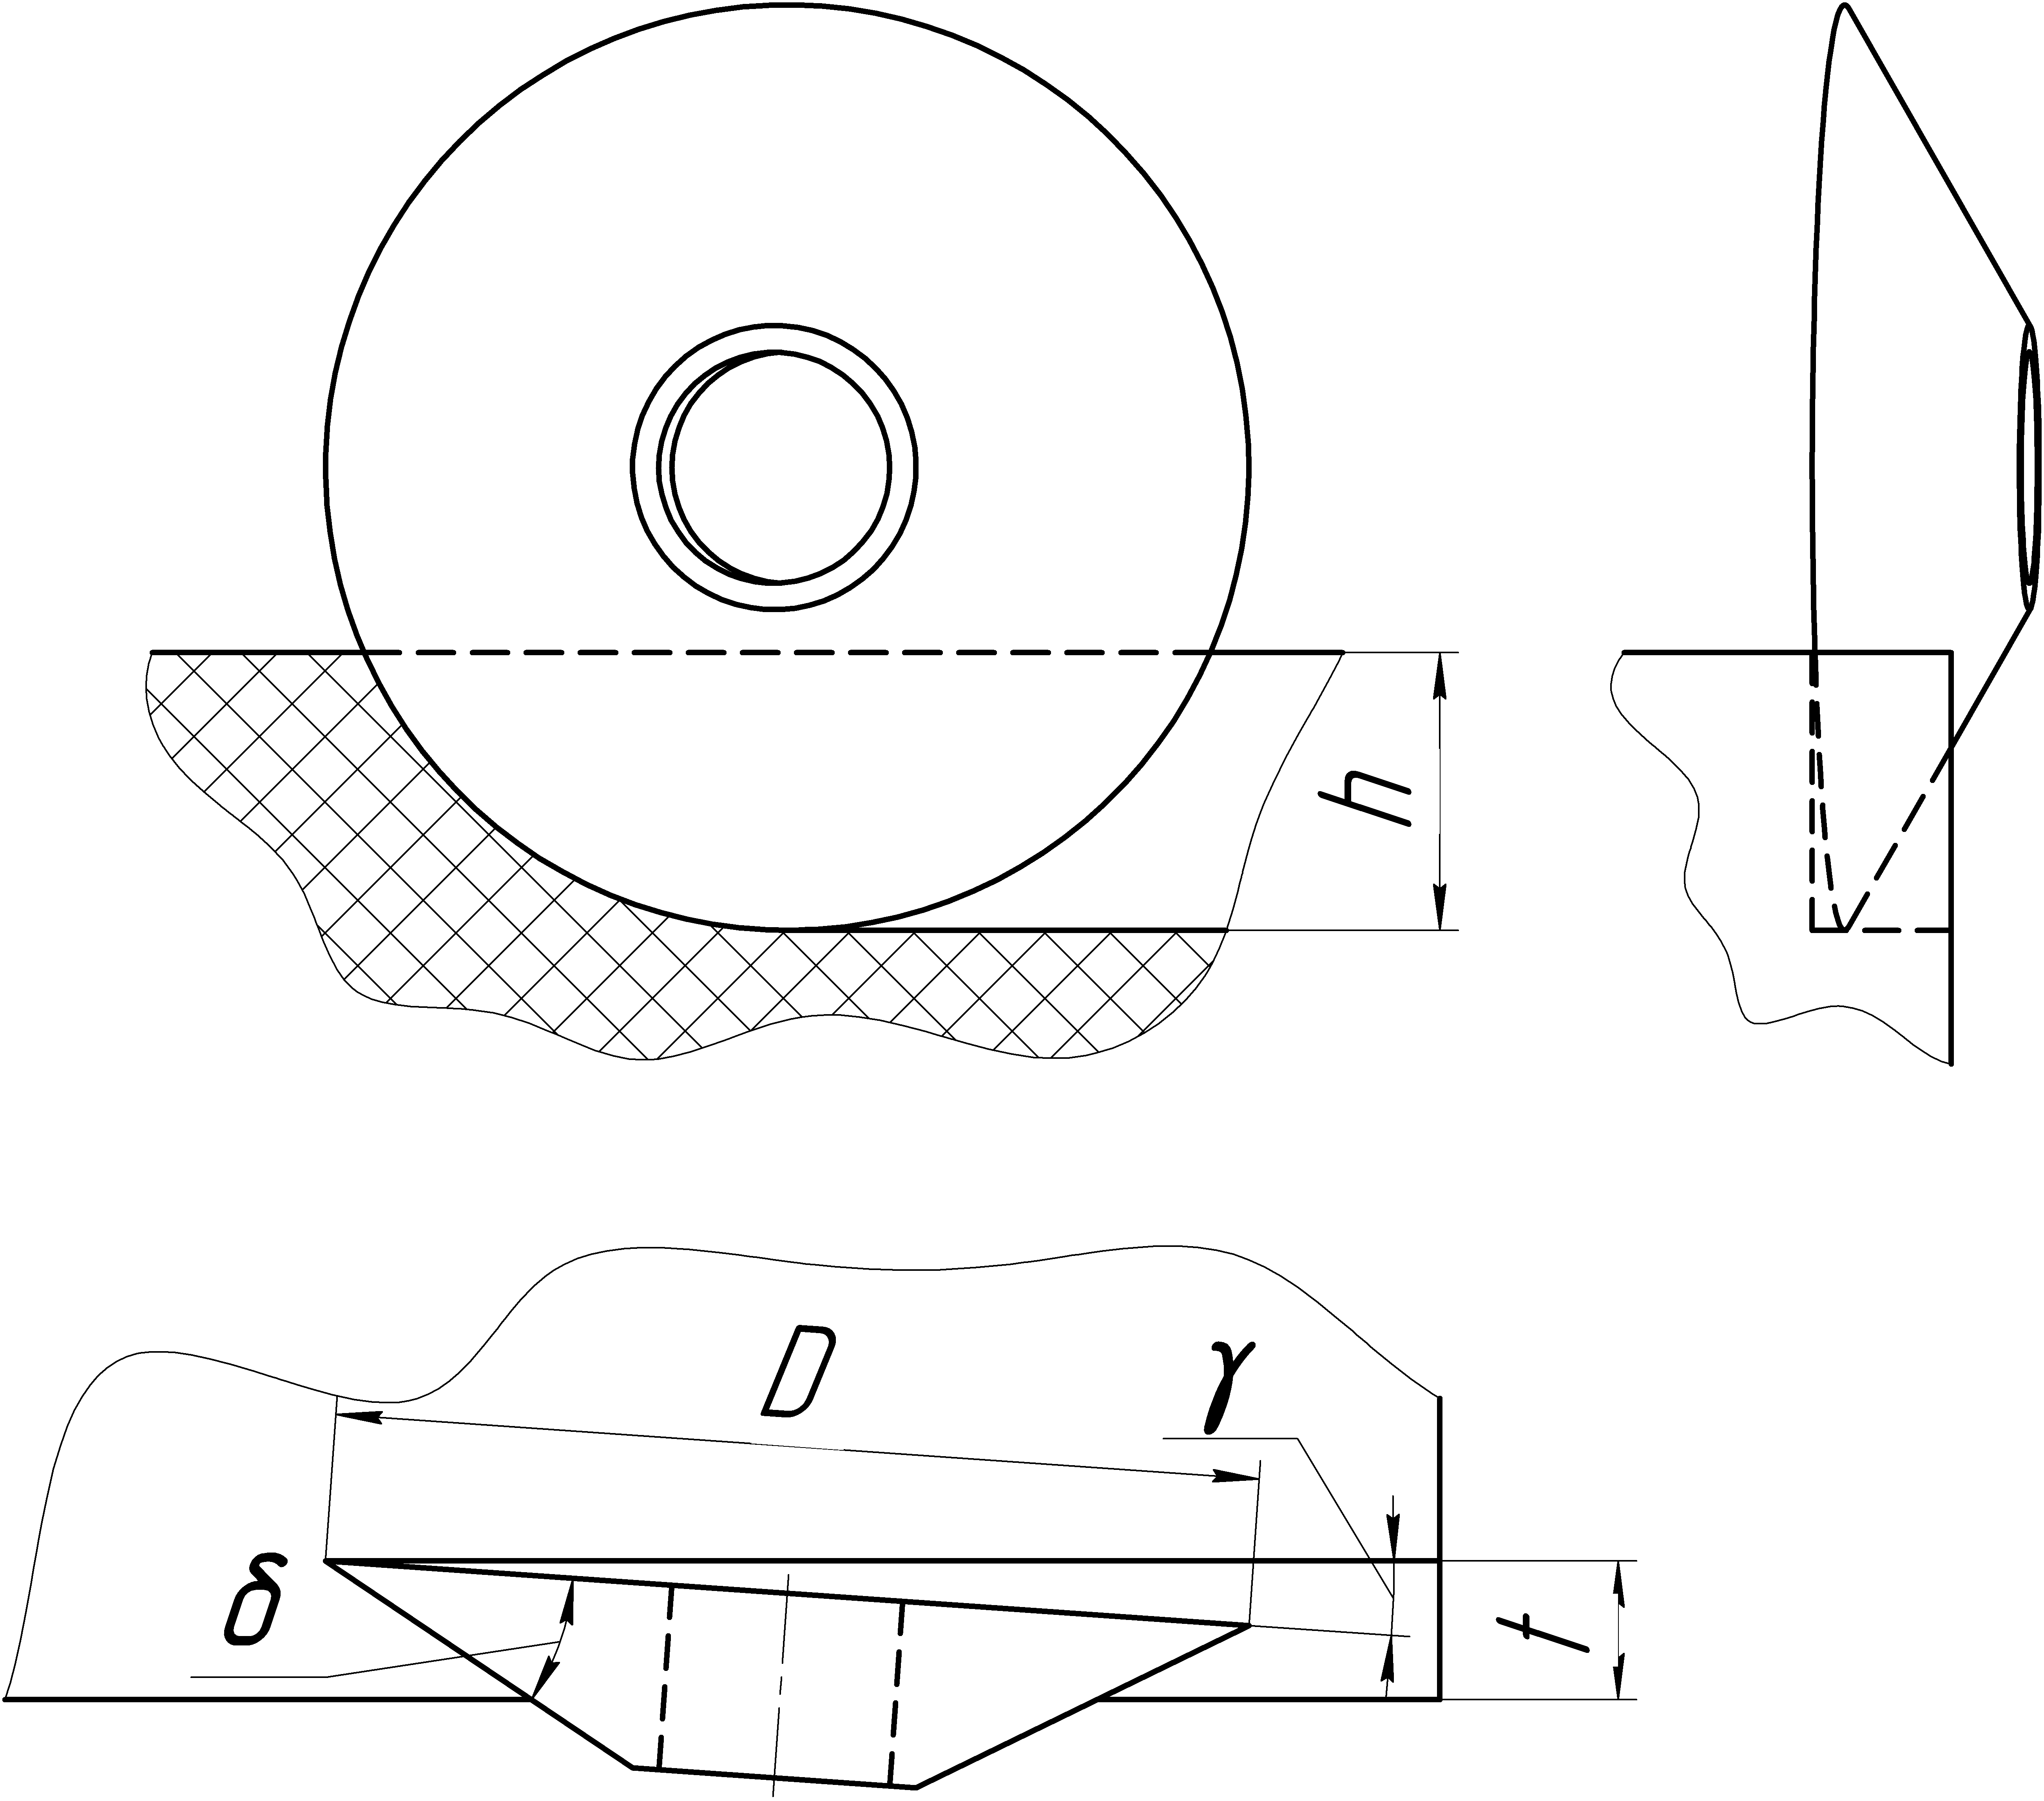
\includegraphics[width=0.5\textwidth]{DRI}

		$t$ "--- шаг резания; $D$ "--- диаметр дискового резца; $\delta$ "--- угол заострения; $h$ "--- глубина резания; $\gamma$ "--- задний угол. 
		\caption{Схема взаимодействия дискового режущего инструмента с разрушаемым массивом} 
		\label{fig:DRI}  
	\end{figure}
	Для более объективного изучения процесса взаимодействия дискового инструмента с ПСЛО предлагается контролировать три составляющие силы резания: горизонтальную, боковую и вертикальную. Контроль этих составляющих непосредственно на рабочем органе мало эффективен, так как: требует больших трудозатрат и дорогостоящего оборудования (датчики силы, оснастка для их монтажа); невозможно изолировать влияние температуры окружающей среды, влажности, теплозапаса дорожного полотна и других факторов друг на друга; постоянно меняются физико-механические свойства ПСЛО (прочность, плотность, наличие абразивного материала). Поэтому, опираясь на работы по резанию мерзлых грунтов различными инструментами \cite{JelukevichGrunt, BaronTang, BaronShar, Zelenin}, целесообразно исследовать процесс взаимодействия полноразмерного дискового режущего инструмента с различным радиусом закругления рабочей кромки с разрушаемым массивом путем стендовых испытаний в лабораторных условиях.
	
	

	При проведении экспериментальных исследований использовались дисковые резцы с различным радиусом закругления рабочей кромки. $ R=[0,5; 1,5; 2,5; 3,5; 4,5] $ мм. Данный диапазон значений обусловлен исследованиями изнашивания режущей кромки проведенными в работе \cite{BaronTang} 

	% \begin{figure}[ht]
	% 	\centering
	% 	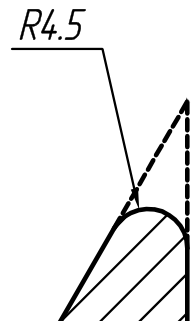
\includegraphics[width=0.2\textwidth]{Radius}
	% 	\caption{Радиус закругления рабочей кромки} 
	% 	\label{fig:Radius}  
	% \end{figure}

	\begin{wrapfigure}{l}{0.3\textwidth}
	  \vspace{-25pt}
	  \begin{center}
	    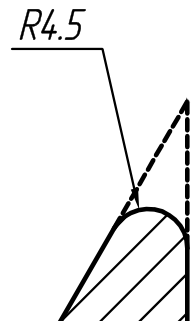
\includegraphics[width=0.2\textwidth]{Radius}
	  \end{center}
	  \vspace{-15pt}
	  \caption{Радиус закругления рабочей кромки}
	  \label{fig:Radius}
	  \vspace{-16pt}
	\end{wrapfigure}

	Остальные параметры дискового режущего инструмента приняты следующими:
	\begin{itemize}
		\item диаметр:  $D=200$ мм.;
		\item угол заострения: $\delta=30^\circ$;
		\item глубина резания: $h=60$ мм.;
		\item шаг резания: $t=[10; 20; 30; 40; 50]$ мм.;
		\item задний угол: $\gamma=3^\circ\div5^\circ$;
		\item температура окружающего воздуха: $-2{}^\circ C\div-7{}^\circ C$;
		\item скорость резания: $0,51\ \slantfrac{\text{м}}{\text{c}}$ ($1,84\ \slantfrac{\text{км}}{\text{ч}}$).
	\end{itemize}

	Для проведения эксперимента использовался механизированный лабораторный стенд описанный в работе \cite{Sram2013Modernizaciya} конструкция которого защищена патентом на изобретение №~2429459 \cite{ExpStend}. Для фиксирования и записи информации применен измерительный комплекс описанный в статье \cite{IKI2016:my}.

	\section{Тензометрический измерительный элемент}

	Тензометрическая балка представляет собой тонкостенную круглую бобышку (рисунок \ref{fig:Zveno}) с прямоугольным основанием, служащим креплением к лабораторному стенду. 


	\begin{wrapfigure}{l}{0.5\textwidth}
	  \vspace{-25pt}
	  \begin{center}
	    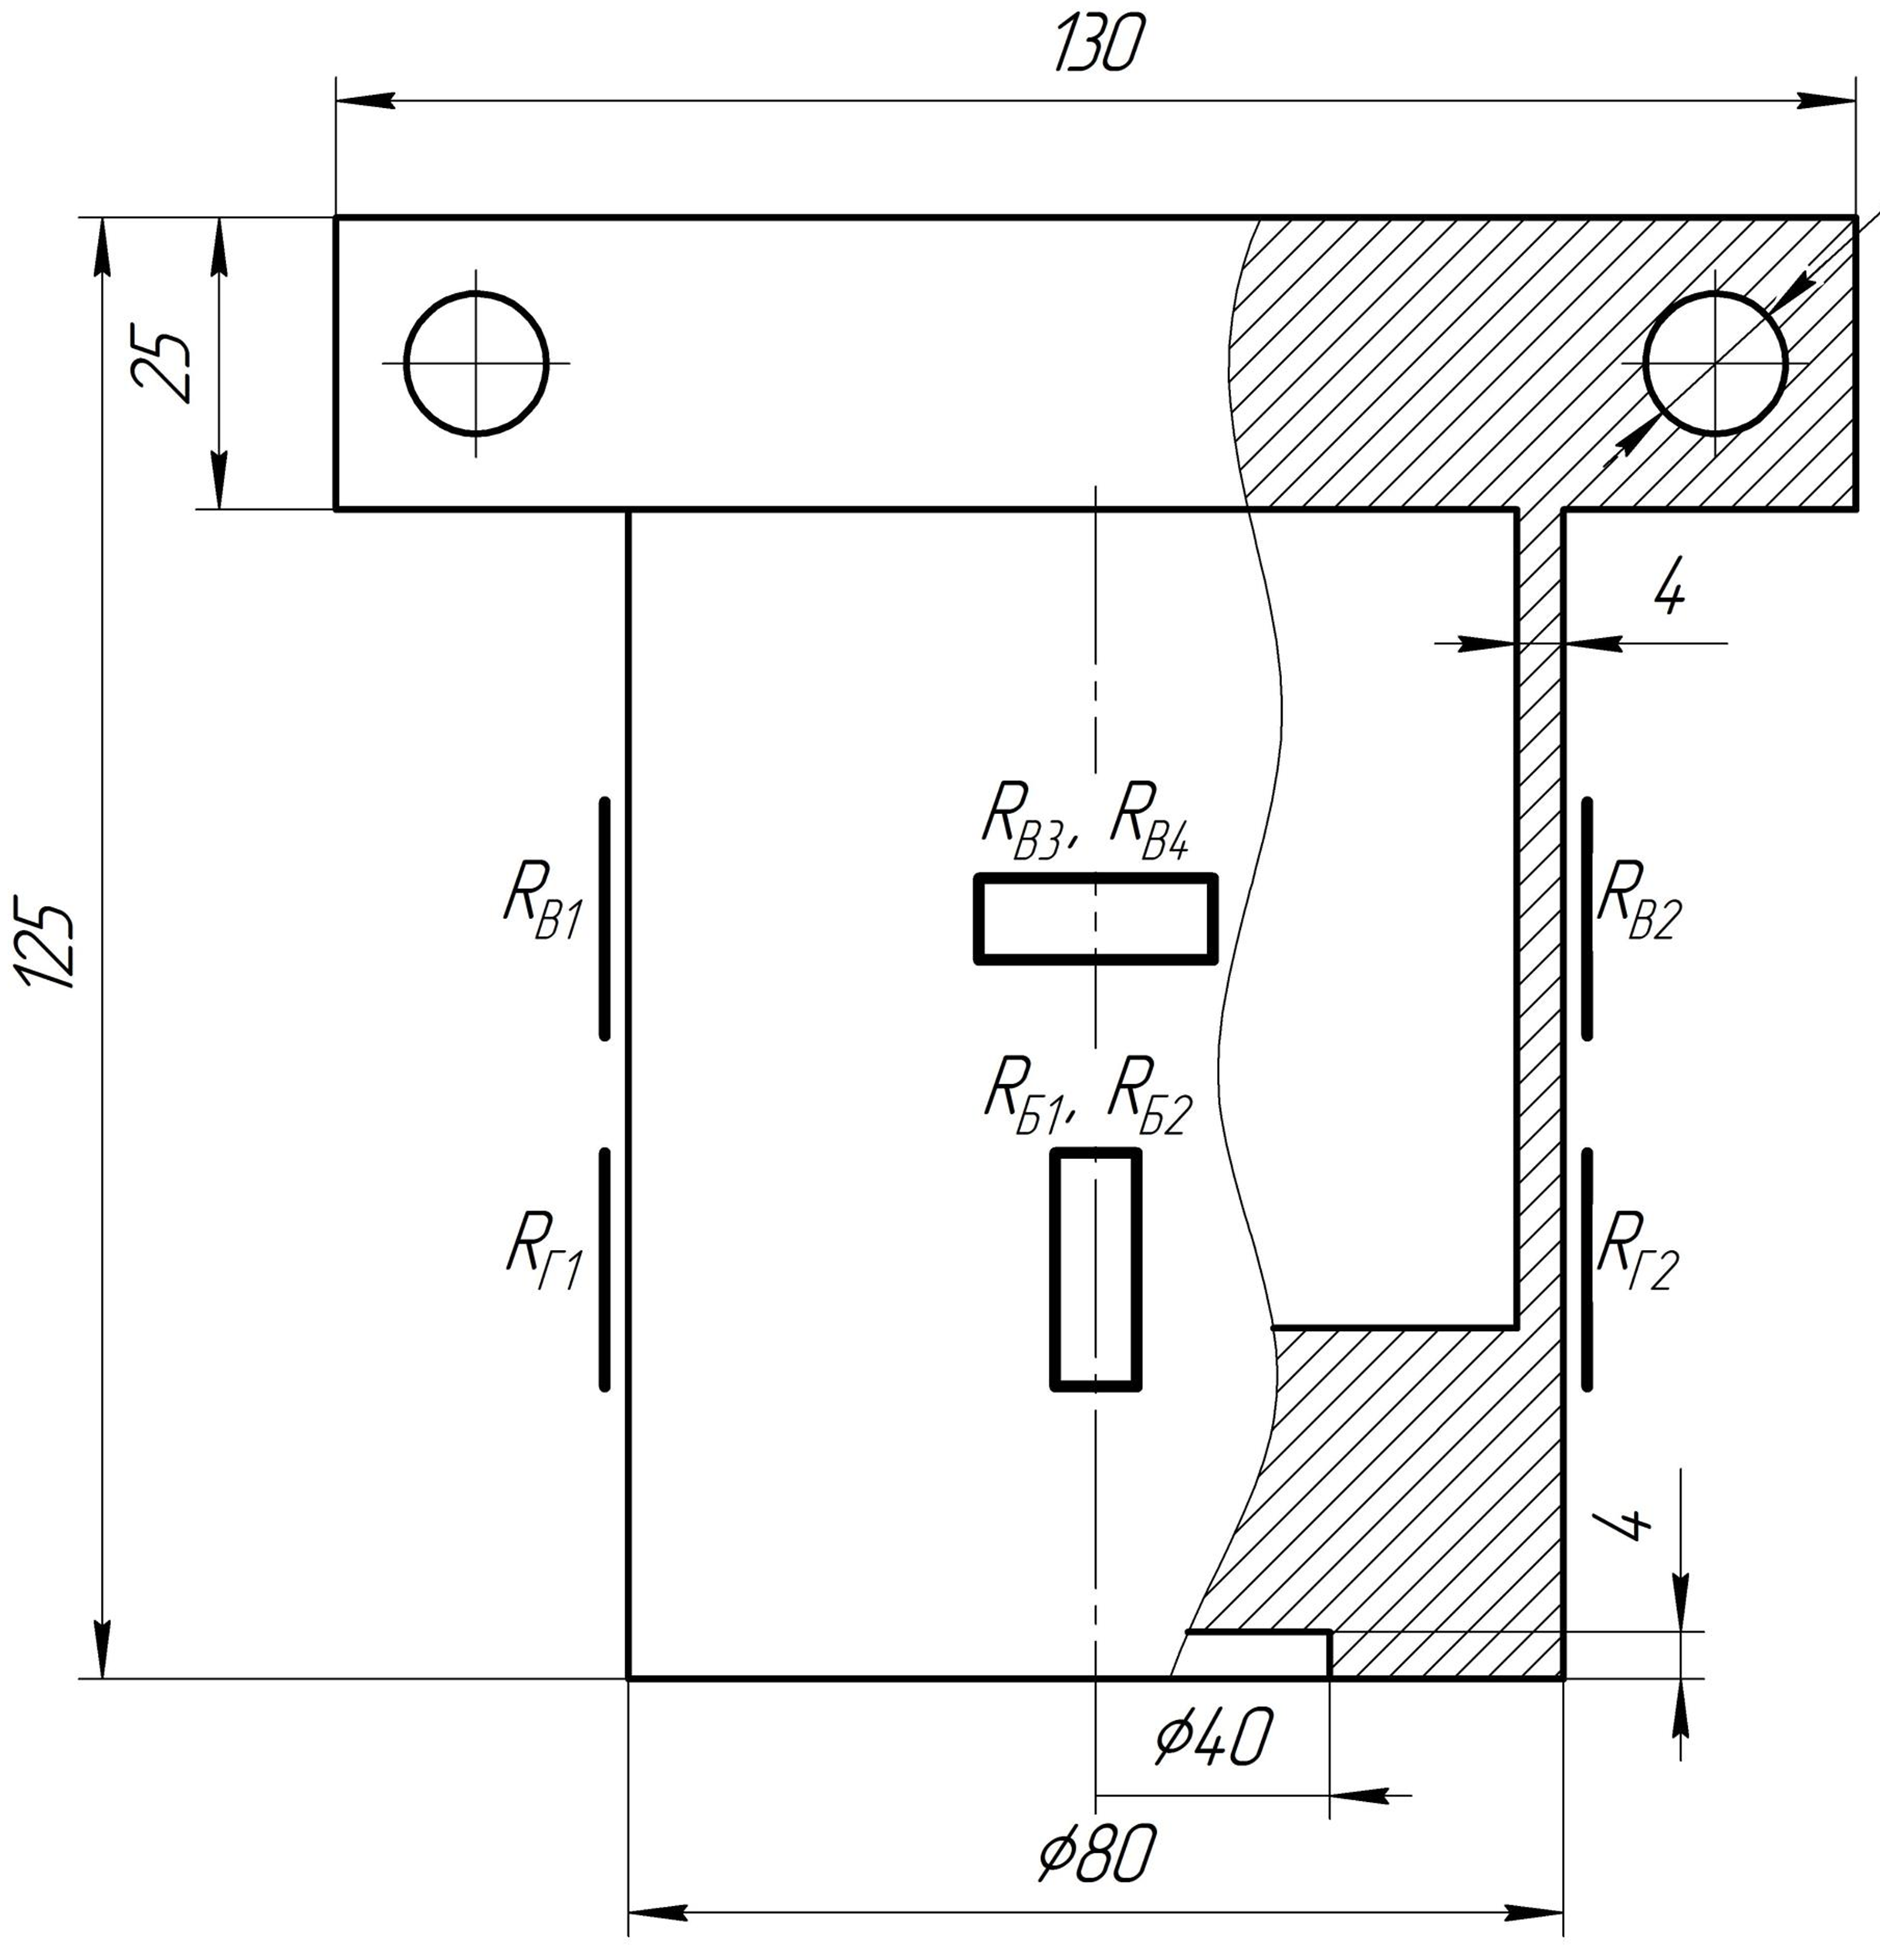
\includegraphics[width=0.5\textwidth]{ZvenoOnli}
	  \end{center}
	  \vspace{-15pt}
	  \caption{Схема наклейки тензорезисторов}
	  \label{fig:Zveno}
	  \vspace{-16pt}
	\end{wrapfigure}


	% \begin{figure}[!h]
	% 	\centering
	% 	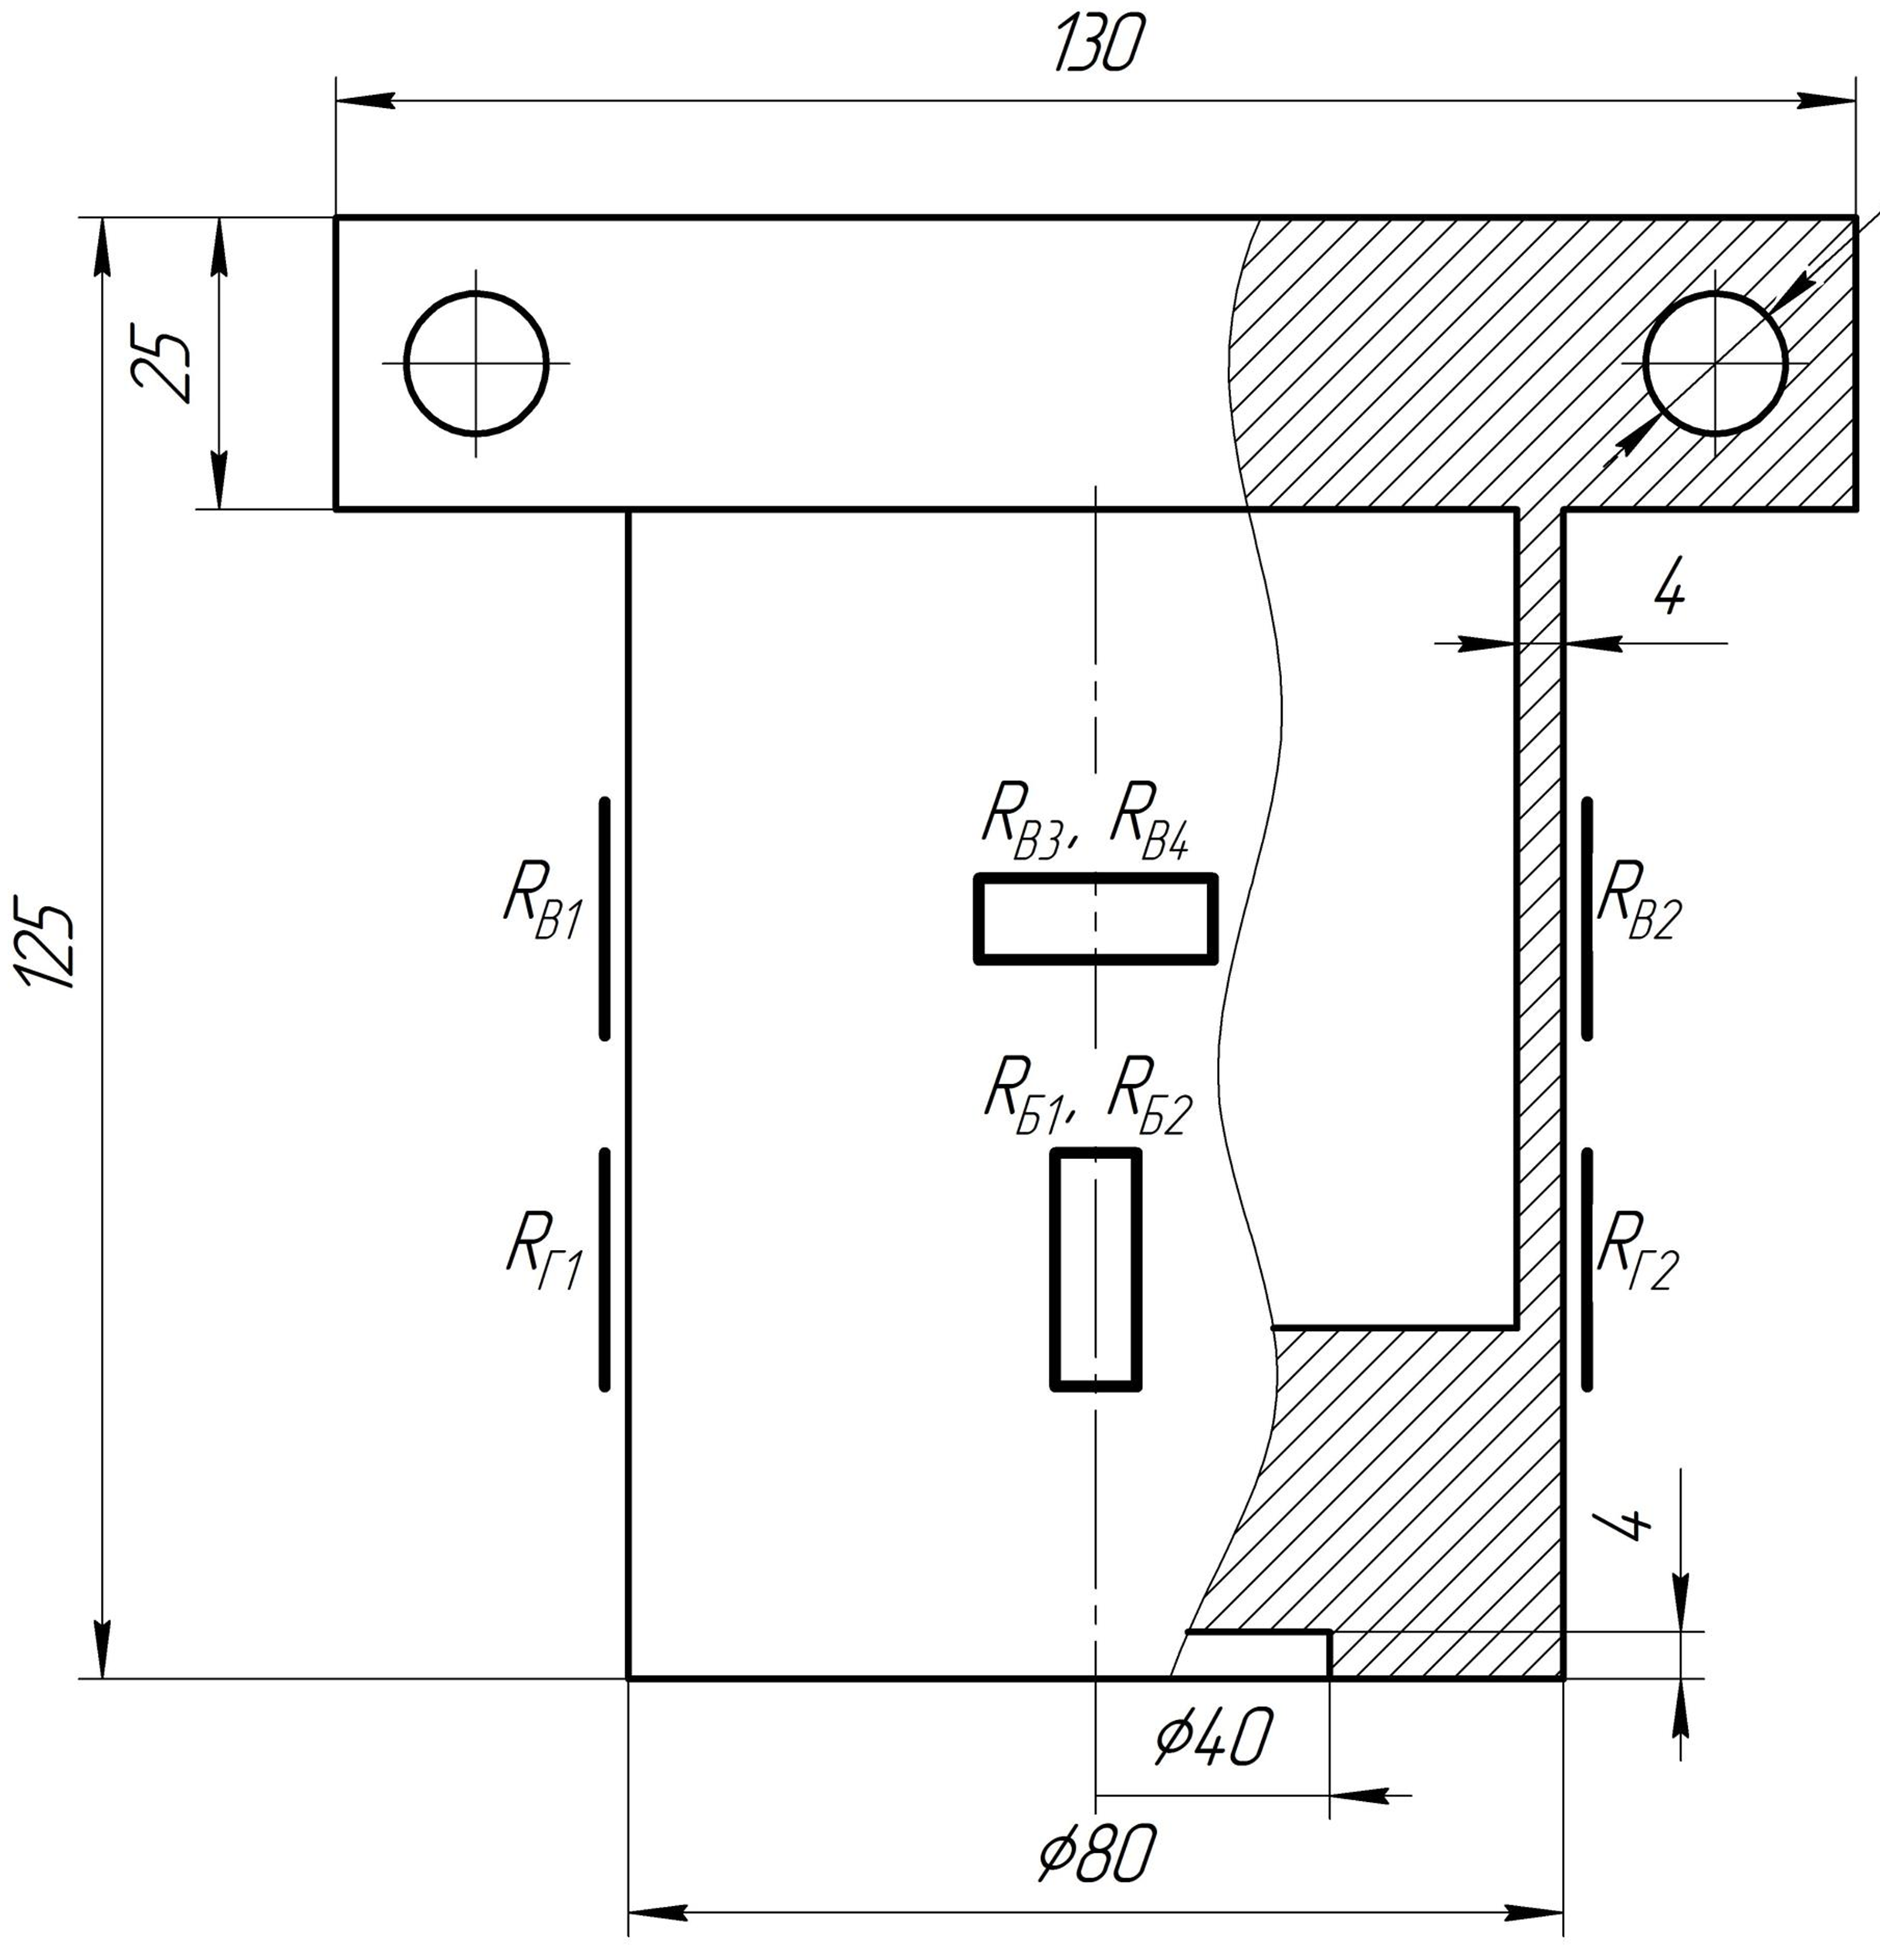
\includegraphics[width=1\textwidth]{ZvenoOnli}
	% 	%
	% 	%А "--- схема наклейки тензорезисторов; Б "--- общий вид тензометрического звена;
	% 	%1 "--- тензометрическая головка; 2 "--- крепёж дискового режущего инструмента
	% 	\caption{Тензометрическое звено} 
	% 	\label{fig:Zveno}  
	% \end{figure}
	Изделие выполнено из стали марки \textit{55С2}. При приложении усилий к такой балке происходит её упругая деформация, которую фиксируют наклеенные на неё тензорезистивные элементы. На рисунке \ref{fig:Zveno} приведена схема наклейки чувствительных элементов.

	Для измерения горизонтальной составляющей приложенного усилия используется полу мостовая схема включения, с избирательной чувствительностью, тензорезистор $R_\textit{Г1}$ включён в первое плечо измерительного моста, а $R_\textit{Г2}$ – в четвёртое. Такая схема позволяет обеспечить избирательную чувствительность тензометрического моста к деформации изгиба (не чувствительна к деформации растяжения-сжатия), возникающей в следствии действия горизонтальной составляющей силы резания. Для боковой составляющей используется схема включения тензорезисторов аналогичная приведённой выше. Тензорезистор $R_\textit{Б1}$ включён в первое плечо измерительного моста, а $R_\textit{Б2}$ – в четвёртое. Для измерения вертикальной составляющей, диаметрально расположенные тензорезисторы $R_\textit{В1}$ и $R_\textit{В2}$ необходимо включить в одно плечо полумоста. Во второе плечо включаются компенсационные тензорезисторы $R_\textit{В3}$ и $R_\textit{В4}$, обеспечивающие также термокомпенсацию. Все схемы включения обеспечивают термокомпенсацию и компенсацию сопротивления соединительных проводов.

	\section{Тарирование тензометрического звена}
	
	Для тарирования тензометрического звена, описанного выше, применялся стенд, конструкция которого защищена патентом на изобретение №~2500983 \cite{CalibrationStend}, позволяющий закреплять звено в различных пространственных положения и соответственно создавать требуемый вектор нагрузки. Тарирование производилось с помощью: одного измерительного прибора "--- динамометра растяжения ДПУ-5-2~5033 второго класса точности; талрепа и вспомогательной оснастки для крепежа тензометрического звена.
	
	Нагрузка звена осуществлялась ступенчато, с шагом 500~Н, до предельного значения в 2~500~Н. Разгрузка производилась с тем же шагом до нулевого значения. На рисунке~\ref{fig:CalibrationRawHor} приведены графики переходных процессов возникающих во время тарирования. Из графиков явно видно, что исключено взаимное влияние составляющих друг на друга.
	
	\begin{figure} [ht]
		\centering
		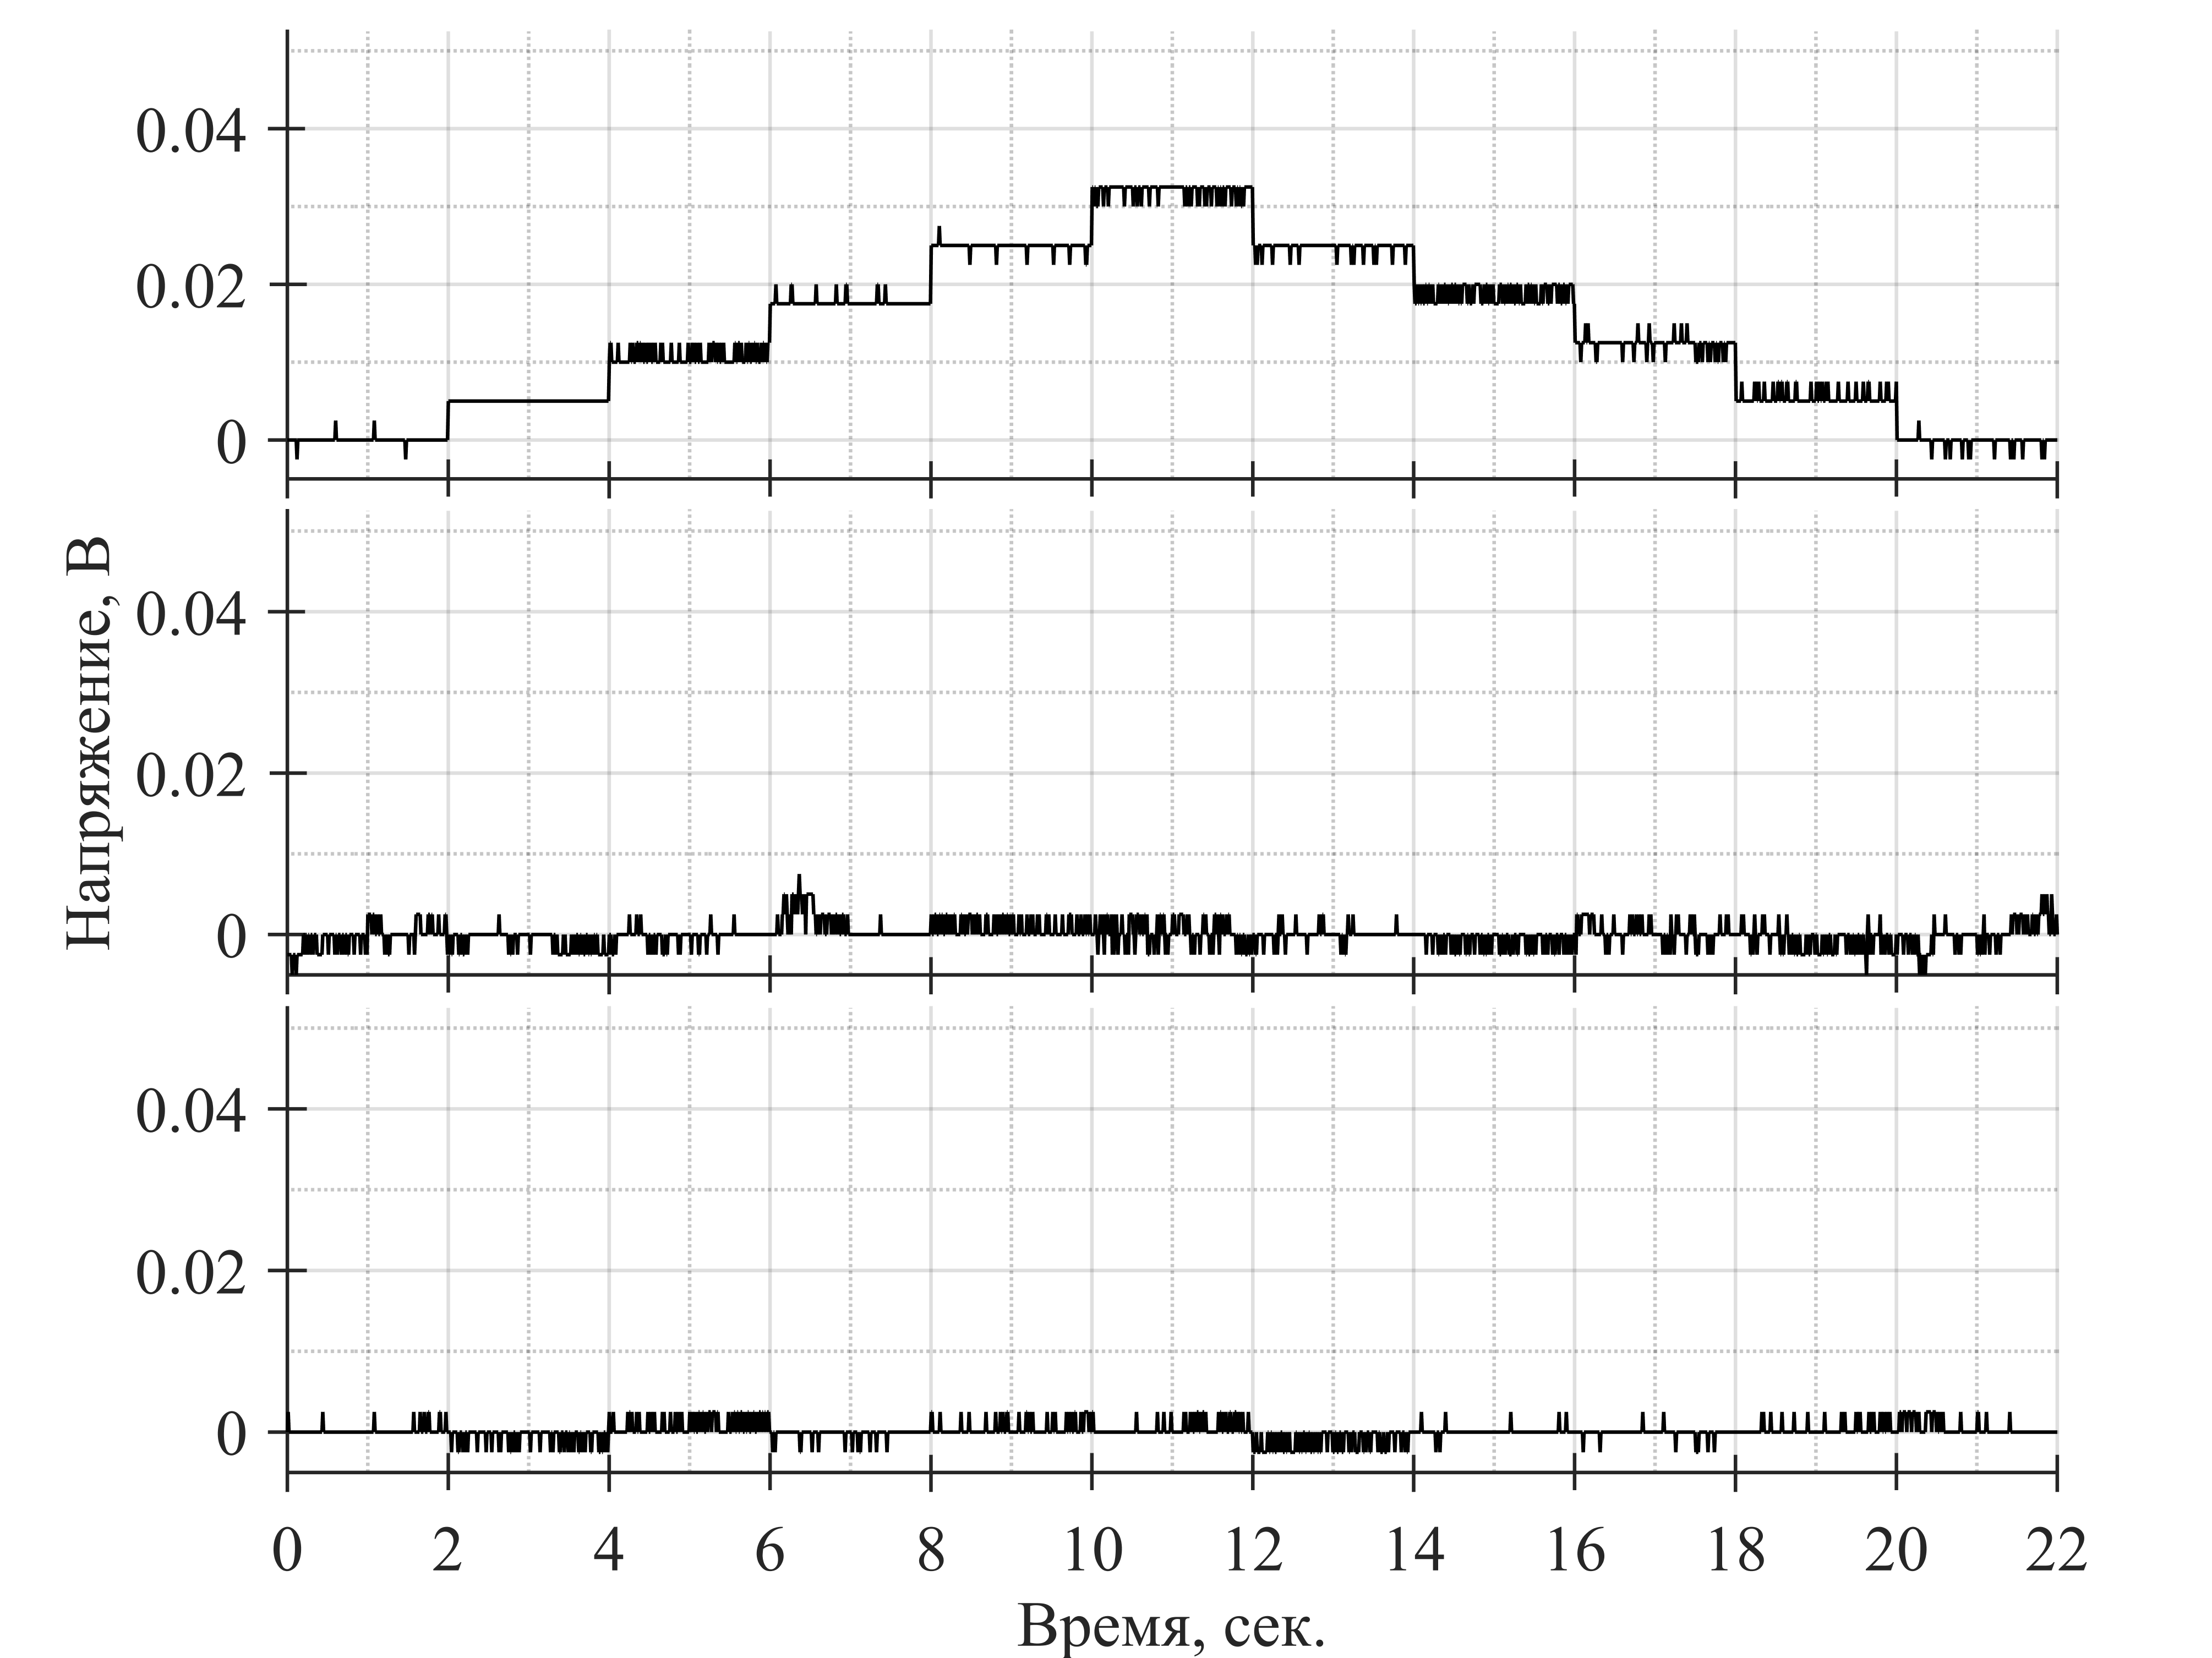
\includegraphics[width=0.7\textwidth]{CalibrationRawHor}
		
		С веху вниз: горизонтальная, боковая, вертикальная составляющие усилия резания
		\caption{Графики переходных процессов при тарировании горизонтальной составляющей усилия резания}  
		\label{fig:CalibrationRawHor}  
	\end{figure}
	
	\begin{table}[htp]
		\centering
		\caption{Зависимость напряжения на каналах оцифровки от приложенной силы в процессе тарирования горизонтальной составляющей усиля резания}
		\label{tab:DCHor}
		\begin{tabular}{|c|c|c|c|}
			\hline
			\multirow{2}{*}{{Сила, Н}} & \multicolumn{3}{c|}{Канал измерения} \tabularnewline
			\cline{2-4}
			                           & {горизонтальный, мВ}                                 & {боковой, мВ} & {вертикальный, мВ}\tabularnewline
			\hline
			\hline
			0                          & 0.0687                                               & 0.175         & 0.325\tabularnewline
			500                        & 5.19                                                 & 0.769         & 0.406\tabularnewline
			1000                       & 11.5                                                 & 0.212         & 0.456\tabularnewline
			1500                       & 18.2                                                 & 0.919         & 0.106\tabularnewline
			2000                       & 24.9                                                 & 0.438         & 0.787\tabularnewline
			2500                       & 32.1                                                 & 0.25          & 0.412\tabularnewline
			\hline
		\end{tabular}
	\end{table}


	Используя данные графиков переходных процессов можно получить зависимости изображенные на рисунке~\ref{fig:Calibration}. Из них видно что силы возникающие на тензометрическом звене имеют линейную зависимость от напряжения получаемого с тензометрических мостов. 

	\begin{figure} [ht]
		\centering
		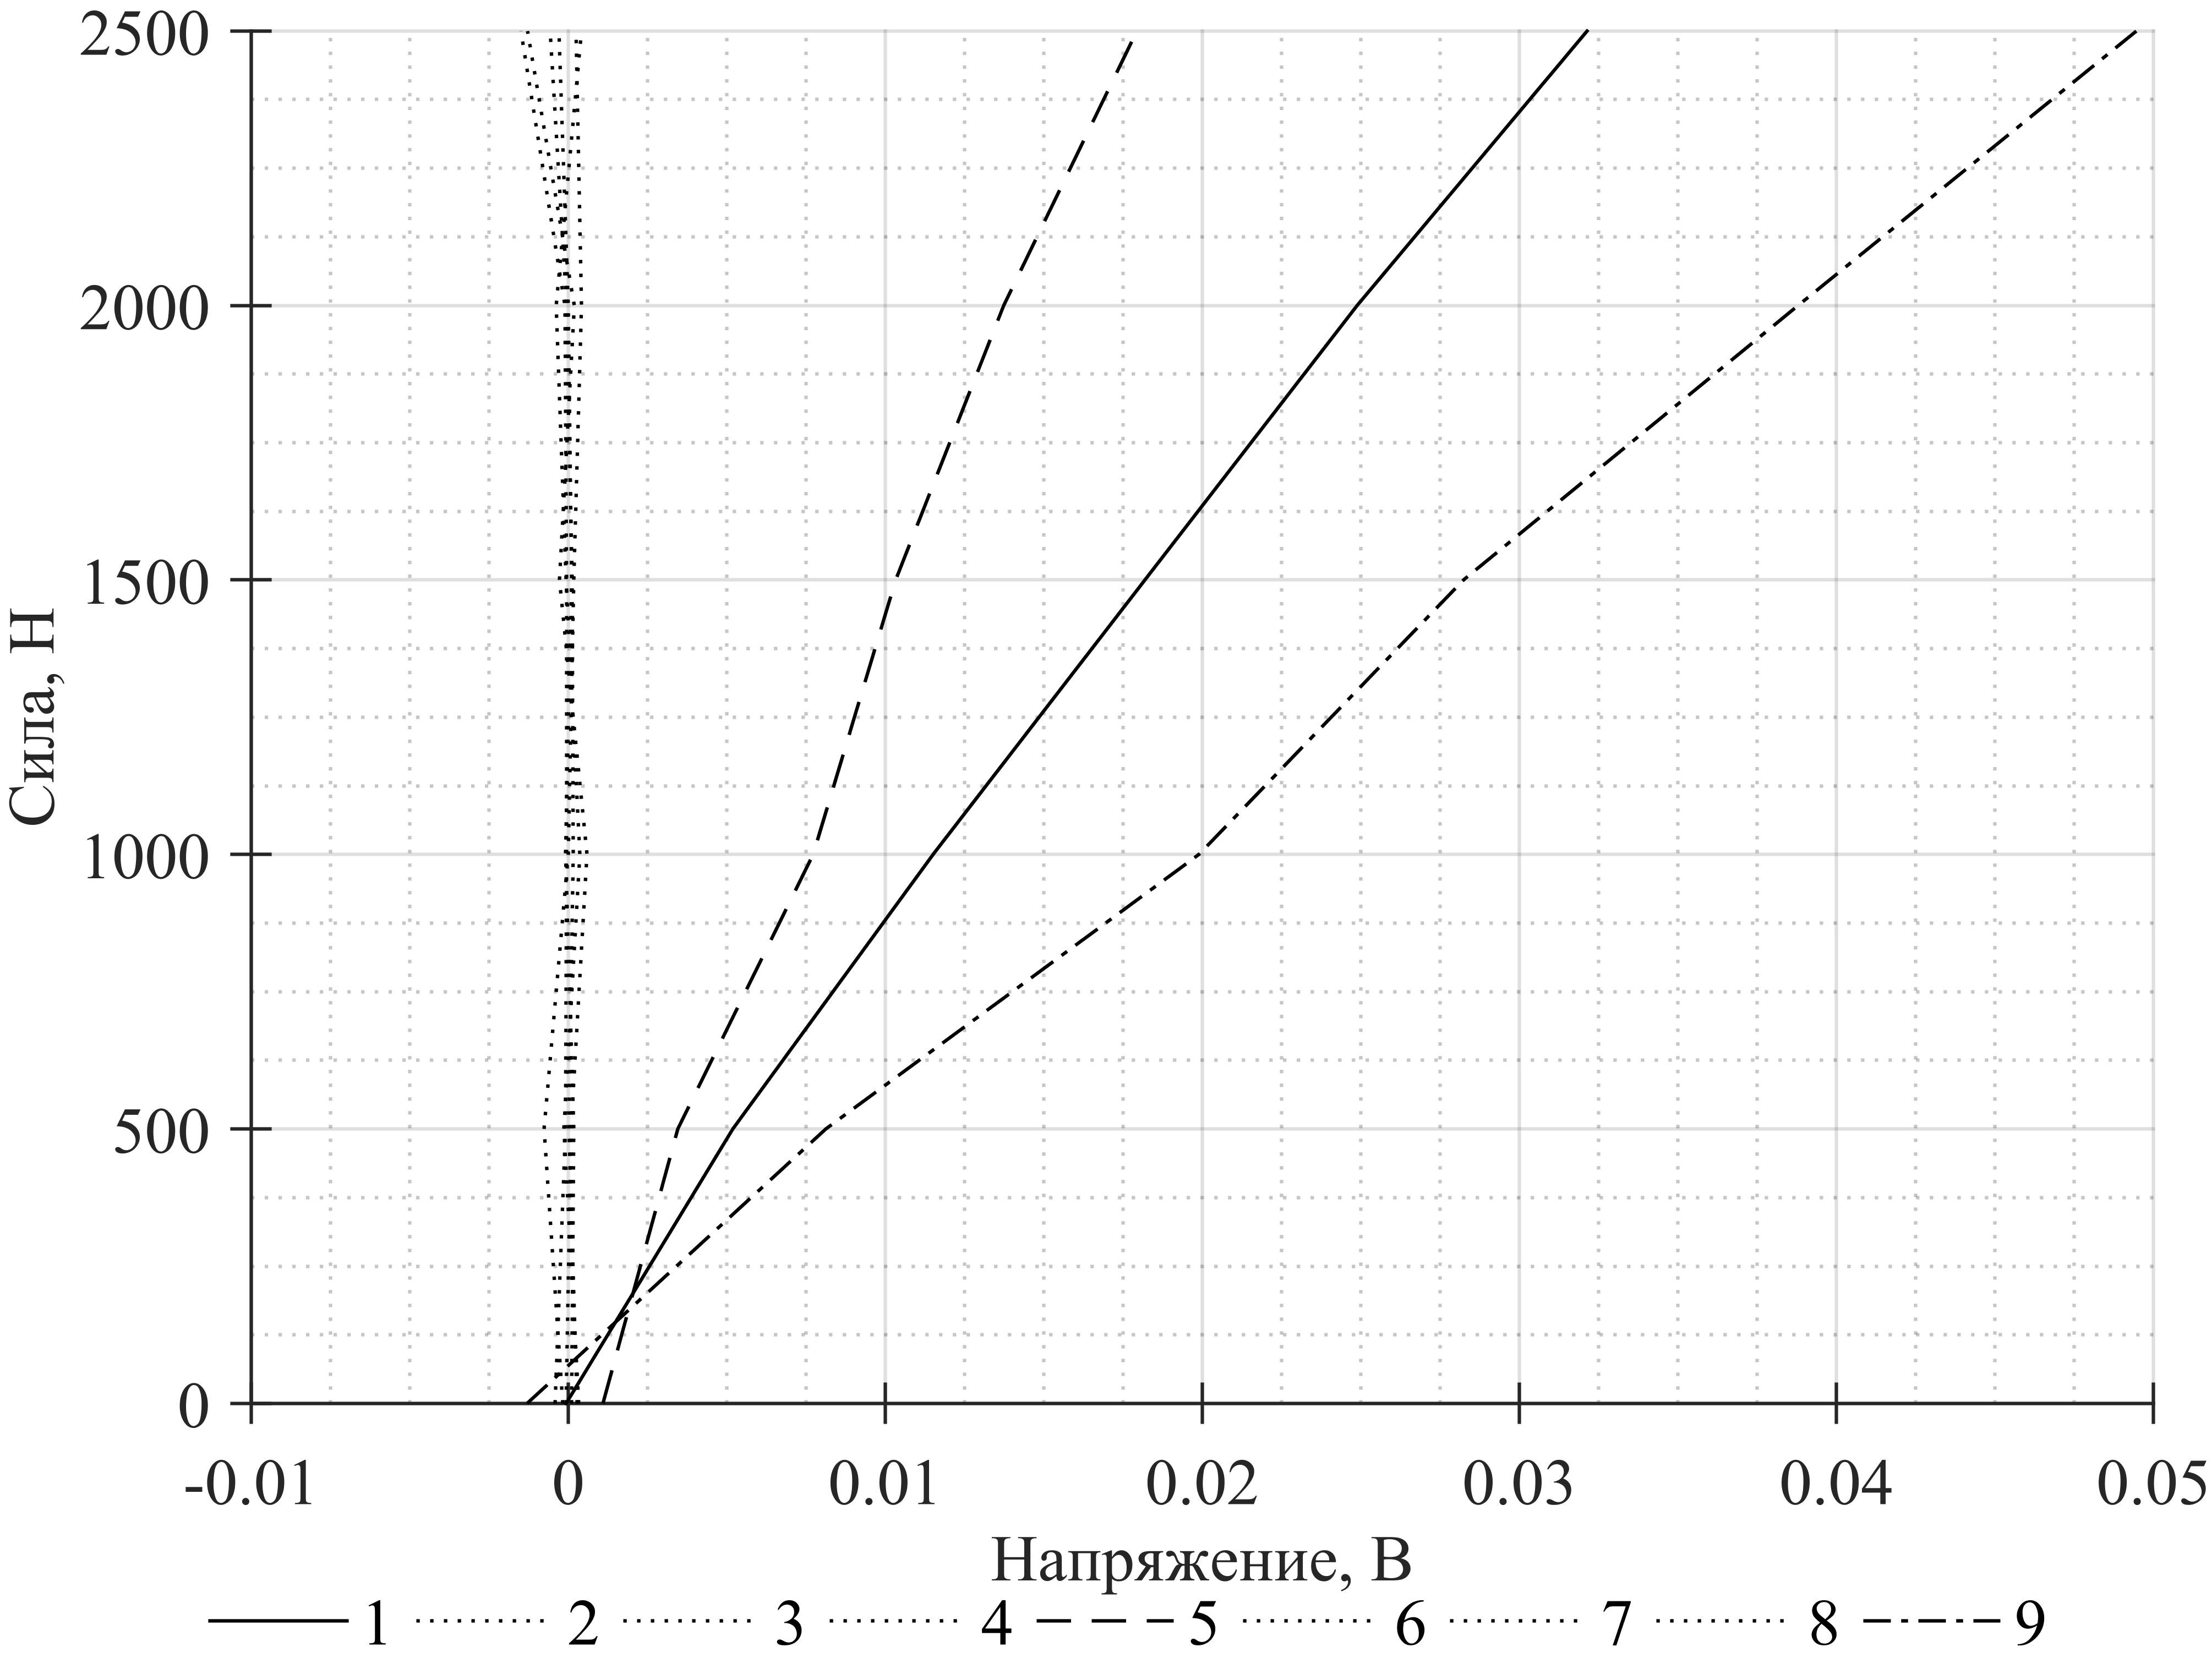
\includegraphics[width=0.7\textwidth]{Calibration.png}
		
		1,2,3 "--- горизонтальная, бокова, вертикальная составляющие усилия резания соответственно при тарировании горизонтальной составляющей; 4,5,6 "--- аналогично  при тарировании боковой составляющей; 7,8,9 "--- аналогично при тарировании вертикальной составляющей.
		\caption{Графики тарирования тензометрического звена}
		\label{fig:Calibration}  
	\end{figure}

	Эти графики можно представить в виде уравнений:
	\begin{align}
		y_\text{гор}  & = 80074.568 \cdot x  \label{eq:TrendHor}\\
		y_\text{бок}  & = 140953.396 \cdot x \label{eq:TrendLat}\\
		y_\text{верт} & = 51338.284 \cdot x \label{eq:TrendVert}
	\end{align}
	Из уравнений \labelcref{eq:TrendHor,eq:TrendLat,eq:TrendVert} получим тарировочные коэффициенты: 8~0074.568~$ \slantfrac{\text{Н}}{\text{В}} $, 140~953.396~$ \slantfrac{\text{Н}}{\text{В}} $, 51~338.284~$ \slantfrac{\text{Н}}{\text{В}} $ для горизонтальной, боковой и вертикальной составляющей усилия резания соответственно.

	\section{Выводы}

	Тарирование следует проводить перед каждой серией экспериментов. Точность тарирования влияет на точность будущих измерений, так как все измерения будут домножены на тарировочный коэффициент. Также в процессе тарирования измерительного преобразователя могут быть выявленны сбои в его работе, поломки. Что позволит своевременно их устранить и обеспечить целостность экспериментальных данных. 

	Тарирование тензометрического звена является одним из важнейших факторов успешности проведения экспериментальных исследований. Известно, что на показания измерительного преобразователя может оказывать влияние множество различных переменных, например: электро магнитные поля; сопротивление проводов; температура окружающей среды. Выявление таких влияний на этапе тарирования измерительного преобразователя, позволяет или полностью их устранить или заложить в тарировочный коэффициент, что в свою очередь сказывается на данных полученных в ходе экспериментальных исследований. 